\documentclass{ximera}

%\usepackage{todonotes}

\newcommand{\todo}{}

\usepackage{tkz-euclide}
\tikzset{>=stealth} %% cool arrow head
\tikzset{shorten <>/.style={ shorten >=#1, shorten <=#1 } } %% allows shorter vectors

\usepackage{tkz-tab}  %% sign charts
\usetikzlibrary{decorations.pathreplacing} 

\usetikzlibrary{backgrounds} %% for boxes around graphs
\usetikzlibrary{shapes,positioning}  %% Clouds and stars
\usetikzlibrary{matrix} %% for matrix
\usepgfplotslibrary{polar} %% for polar plots
\usetkzobj{all}
\usepackage[makeroom]{cancel} %% for strike outs
%\usepackage{mathtools} %% for pretty underbrace % Breaks Ximera
\usepackage{multicol}

\usepackage{polynom}



\usepackage[many]{tcolorbox}  %% for titled boxes
\newtcolorbox{xbox}[1]{%
    tikznode boxed title,
    enhanced,
    arc=0mm,
    interior style={white},
    attach boxed title to top center= {yshift=-\tcboxedtitleheight/2},
    fonttitle=\bfseries,
    colbacktitle=white,coltitle=black,
    boxed title style={size=normal,colframe=white,boxrule=0pt},
    title={#1}}


\usepackage{array}
\setlength{\extrarowheight}{+.1cm}   
\newdimen\digitwidth
\settowidth\digitwidth{9}
\def\divrule#1#2{
\noalign{\moveright#1\digitwidth
\vbox{\hrule width#2\digitwidth}}}





\newcommand{\RR}{\mathbb R}
\newcommand{\R}{\mathbb R}
\newcommand{\N}{\mathbb N}
\newcommand{\Z}{\mathbb Z}

%\renewcommand{\d}{\,d\!}
\renewcommand{\d}{\mathop{}\!d}
\newcommand{\dd}[2][]{\frac{\d #1}{\d #2}}
\newcommand{\pp}[2][]{\frac{\partial #1}{\partial #2}}
\renewcommand{\l}{\ell}
\newcommand{\ddx}{\frac{d}{\d x}}
\newcommand{\ddt}{\frac{d}{\d t}}

\newcommand{\zeroOverZero}{\ensuremath{\boldsymbol{\tfrac{0}{0}}}}
\newcommand{\inftyOverInfty}{\ensuremath{\boldsymbol{\tfrac{\infty}{\infty}}}}
\newcommand{\zeroOverInfty}{\ensuremath{\boldsymbol{\tfrac{0}{\infty}}}}
\newcommand{\zeroTimesInfty}{\ensuremath{\small\boldsymbol{0\cdot \infty}}}
\newcommand{\inftyMinusInfty}{\ensuremath{\small\boldsymbol{\infty - \infty}}}
\newcommand{\oneToInfty}{\ensuremath{\boldsymbol{1^\infty}}}
\newcommand{\zeroToZero}{\ensuremath{\boldsymbol{0^0}}}
\newcommand{\inftyToZero}{\ensuremath{\boldsymbol{\infty^0}}}



\newcommand{\numOverZero}{\ensuremath{\boldsymbol{\tfrac{\#}{0}}}}
\newcommand{\dfn}{\textbf}
%\newcommand{\unit}{\,\mathrm}
\newcommand{\unit}{\mathop{}\!\mathrm}
\newcommand{\eval}[1]{\bigg[ #1 \bigg]}
\newcommand{\seq}[1]{\left( #1 \right)}
\renewcommand{\epsilon}{\varepsilon}
\renewcommand{\iff}{\Leftrightarrow}

\DeclareMathOperator{\arccot}{arccot}
\DeclareMathOperator{\arcsec}{arcsec}
\DeclareMathOperator{\arccsc}{arccsc}
\DeclareMathOperator{\si}{Si}
\DeclareMathOperator{\proj}{proj}
\DeclareMathOperator{\scal}{scal}


\newcommand{\tightoverset}[2]{% for arrow vec
  \mathop{#2}\limits^{\vbox to -.5ex{\kern-0.75ex\hbox{$#1$}\vss}}}
\newcommand{\arrowvec}[1]{\tightoverset{\scriptstyle\rightharpoonup}{#1}}
\renewcommand{\vec}{\mathbf}
\newcommand{\veci}{\vec{i}}
\newcommand{\vecj}{\vec{j}}
\newcommand{\veck}{\vec{k}}
\newcommand{\vecl}{\boldsymbol{\l}}

\newcommand{\dotp}{\bullet}
\newcommand{\cross}{\boldsymbol\times}
\newcommand{\grad}{\boldsymbol\nabla}
\newcommand{\divergence}{\grad\dotp}
\newcommand{\curl}{\grad\cross}
%\DeclareMathOperator{\divergence}{divergence}
%\DeclareMathOperator{\curl}[1]{\grad\cross #1}


\colorlet{textColor}{black} 
\colorlet{background}{white}
\colorlet{penColor}{blue!50!black} % Color of a curve in a plot
\colorlet{penColor2}{red!50!black}% Color of a curve in a plot
\colorlet{penColor3}{red!50!blue} % Color of a curve in a plot
\colorlet{penColor4}{green!50!black} % Color of a curve in a plot
\colorlet{penColor5}{orange!80!black} % Color of a curve in a plot
\colorlet{fill1}{penColor!20} % Color of fill in a plot
\colorlet{fill2}{penColor2!20} % Color of fill in a plot
\colorlet{fillp}{fill1} % Color of positive area
\colorlet{filln}{penColor2!20} % Color of negative area
\colorlet{fill3}{penColor3!20} % Fill
\colorlet{fill4}{penColor4!20} % Fill
\colorlet{fill5}{penColor5!20} % Fill
\colorlet{gridColor}{gray!50} % Color of grid in a plot

\newcommand{\surfaceColor}{violet}
\newcommand{\surfaceColorTwo}{redyellow}
\newcommand{\sliceColor}{greenyellow}




\pgfmathdeclarefunction{gauss}{2}{% gives gaussian
  \pgfmathparse{1/(#2*sqrt(2*pi))*exp(-((x-#1)^2)/(2*#2^2))}%
}


%%%%%%%%%%%%%
%% Vectors
%%%%%%%%%%%%%

%% Simple horiz vectors
\renewcommand{\vector}[1]{\left\langle #1\right\rangle}


%% %% Complex Horiz Vectors with angle brackets
%% \makeatletter
%% \renewcommand{\vector}[2][ , ]{\left\langle%
%%   \def\nextitem{\def\nextitem{#1}}%
%%   \@for \el:=#2\do{\nextitem\el}\right\rangle%
%% }
%% \makeatother

%% %% Vertical Vectors
%% \def\vector#1{\begin{bmatrix}\vecListA#1,,\end{bmatrix}}
%% \def\vecListA#1,{\if,#1,\else #1\cr \expandafter \vecListA \fi}

%%%%%%%%%%%%%
%% End of vectors
%%%%%%%%%%%%%

%\newcommand{\fullwidth}{}
%\newcommand{\normalwidth}{}



%% makes a snazzy t-chart for evaluating functions
%\newenvironment{tchart}{\rowcolors{2}{}{background!90!textColor}\array}{\endarray}

%%This is to help with formatting on future title pages.
\newenvironment{sectionOutcomes}{}{} 



%% Flowchart stuff
%\tikzstyle{startstop} = [rectangle, rounded corners, minimum width=3cm, minimum height=1cm,text centered, draw=black]
%\tikzstyle{question} = [rectangle, minimum width=3cm, minimum height=1cm, text centered, draw=black]
%\tikzstyle{decision} = [trapezium, trapezium left angle=70, trapezium right angle=110, minimum width=3cm, minimum height=1cm, text centered, draw=black]
%\tikzstyle{question} = [rectangle, rounded corners, minimum width=3cm, minimum height=1cm,text centered, draw=black]
%\tikzstyle{process} = [rectangle, minimum width=3cm, minimum height=1cm, text centered, draw=black]
%\tikzstyle{decision} = [trapezium, trapezium left angle=70, trapezium right angle=110, minimum width=3cm, minimum height=1cm, text centered, draw=black]


\outcome{Find the intervals where a function is increasing or decreasing.}
\outcome{Find the intervals where a function is concave up or down.}
\outcome{Find any asymptotic behaviors a function may have: vertical, horizontal, or slant.}
\outcome{Determine how the graph of a function looks without using a calculator.}

\author{Nela Lakos \and Kyle Parsons}

\begin{document}
\begin{exercise}

Consider the function $f(x) = \frac{3x^5-20x^3}{32}$.

The domain of $f$ is $\left(\answer{-\infty},\answer{\infty}\right)$.

$f$ is \wordChoice{\choice{even}\choice[correct]{odd}\choice{neither even nor odd}}.

$f$ \wordChoice{\choice{has}\choice[correct]{has no}} horizontal asymptotes.

$f$ \wordChoice{\choice{has}\choice[correct]{has no}} vertical asymptotes.

The derivative of $f$ is given by
\[
f'(x) = \answer{\frac{15x^2(x-2)(x+2)}{32}}.
\]

The second derivative of $f$ is given by 
\[
f''(x) = \answer{\frac{15x(x-\sqrt{2})(x+\sqrt{2})}{8}}.
\]

$f$ is increasing and concave down on $\left(\answer{-\infty},\answer{-2}\right)$.

$f$ is increasing and concave up on $\left(\answer{2},\answer{\infty}\right)$.

$f$ is decreasing and concave down on (from left to right) $\left(\answer{-2},\answer{-\sqrt{2}}\right)$ and $\left(\answer{0},\answer{\sqrt{2}}\right)$.

$f$ is decreasing and concave down on (from left to right) $\left(\answer{-\sqrt{2}},\answer{0}\right)$ and $\left(\answer{\sqrt{2}},\answer{2}\right)$.

$f$ achieves a local minimum at $x=\answer{2}$.

$f$ achieves a local maximum at $x=\answer{-2}$.

$f$ has inflection points (from left to right) at $x=\answer{-\sqrt{2}}$, $x=\answer{0}$ and $x=\answer{\sqrt{2}}$.

Consider the graphs below.

\resizebox{0.45\textwidth}{!}{
  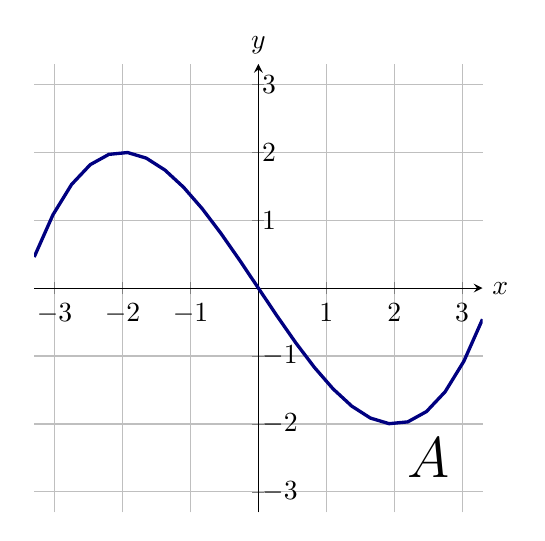
\begin{tikzpicture}
    \begin{axis}[
        xmin=-3.3,xmax=3.3,ymin=-3.3,ymax=3.3,
        clip=true,
        unit vector ratio*=1 1 1,
        axis lines=center,
        grid = major,
        ytick={-20,-19,...,20},
        xtick={-20,-19,...,20},
        xlabel=$x$, ylabel=$y$,
        y tick label style={anchor=west},
        every axis y label/.style={at=(current axis.above origin),anchor=south},
        every axis x label/.style={at=(current axis.right of origin),anchor=west},
      ]
      \addplot[very thick,penColor,domain=-3.3:3.3] plot{(x^3/12-x)*3/2};

      \node at (axis cs:2.5,-2.5) {\huge $A$};
      \end{axis}`
  \end{tikzpicture}}
\hfill
\resizebox{0.45\textwidth}{!}{
  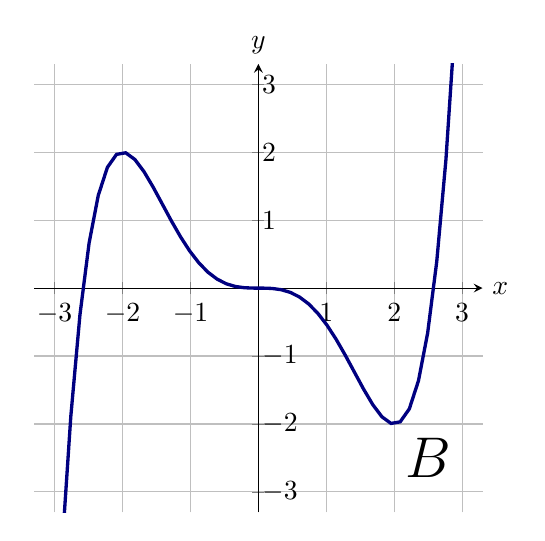
\begin{tikzpicture}
    \begin{axis}[
        xmin=-3.3,xmax=3.3,ymin=-3.3,ymax=3.3,
        clip=true,
        unit vector ratio*=1 1 1,
        axis lines=center,
        grid = major,
        ytick={-20,-19,...,20},
        xtick={-20,-19,...,20},
        xlabel=$x$, ylabel=$y$,
        y tick label style={anchor=west},
        every axis y label/.style={at=(current axis.above origin),anchor=south},
        every axis x label/.style={at=(current axis.right of origin),anchor=west},
      ]
      \addplot[very thick,penColor,domain=-3.3:3.3,samples=50] plot{(3*x^5-20*x^3)/32};
      
      \node at (axis cs:2.5,-2.5) {\huge $B$};
      \end{axis}`
  \end{tikzpicture}}

\resizebox{0.45\textwidth}{!}{
  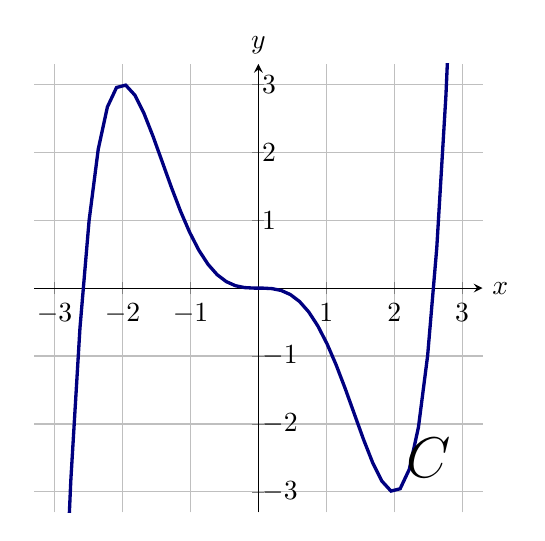
\begin{tikzpicture}
    \begin{axis}[
        xmin=-3.3,xmax=3.3,ymin=-3.3,ymax=3.3,
        clip=true,
        unit vector ratio*=1 1 1,
        axis lines=center,
        grid = major,
        ytick={-20,-19,...,20},
        xtick={-20,-19,...,20},
        xlabel=$x$, ylabel=$y$,
        y tick label style={anchor=west},
        every axis y label/.style={at=(current axis.above origin),anchor=south},
        every axis x label/.style={at=(current axis.right of origin),anchor=west},
      ]
      \addplot[very thick,penColor,domain=-3.3:3.3,samples=50] plot{(3*x^5-20*x^3)*3/64};
            
      \node at (axis cs:2.5,-2.5) {\huge $C$};
      \end{axis}`
  \end{tikzpicture}}
\hfill
\resizebox{0.45\textwidth}{!}{
  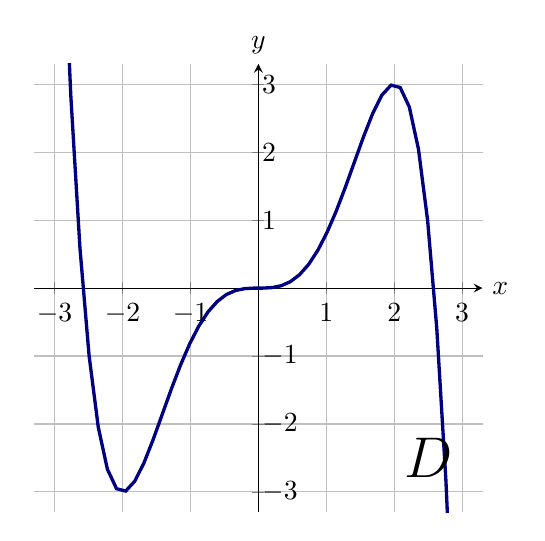
\begin{tikzpicture}
    \begin{axis}[
        xmin=-3.3,xmax=3.3,ymin=-3.3,ymax=3.3,
        clip=true,
        unit vector ratio*=1 1 1,
        axis lines=center,
        grid = major,
        ytick={-20,-19,...,20},
        xtick={-20,-19,...,20},
        xlabel=$x$, ylabel=$y$,
        y tick label style={anchor=west},
        every axis y label/.style={at=(current axis.above origin),anchor=south},
        every axis x label/.style={at=(current axis.right of origin),anchor=west},
      ]
      \addplot[very thick,penColor,domain=-3.3:3.3,samples=50] plot{(3*(-x)^5-20*(-x)^3)*3/64};
            
      \node at (axis cs:2.5,-2.5) {\huge $D$};
      \end{axis}`
  \end{tikzpicture}}

Chose the graph that correctly depicts $f(x)$.
\begin{multipleChoice}
\choice{$A$}
\choice[correct]{$B$}
\choice{$C$}
\choice{$D$}
\end{multipleChoice}


\end{exercise}
\end{document}